\documentclass[table]{beamer}
%[]中可以使用draft、handout、screen、transparency、trancompress、compress等参数

%指定beamer的模式与主题
\mode<presentation>
{
  \usetheme{Madrid}
%\usetheme{Boadilla}
%\usecolortheme{default}
%\usecolortheme{orchid}
%\usecolortheme{whale}
%\usefonttheme{professionalfonts}
}

%\usetheme{Madrid}
%这里还可以选择别的主题:Bergen, Boadilla, Madrid, AnnArbor, CambridgeUS, Pittsburgh, Rochester, Warsaw, ...
%有导航栏的Antibes, JuanLesPins, Montpellier, ...
%有内容的Berkeley, PaloAlto, Goettingen, Marburg, Hannover, ...
%有最小导航栏的Berlin, Ilmenau, Dresden, Darmstadt, Frankfurt, Singapore, Szeged, ...
%有章和节表单的Copenhagen, Luebeck, Malmoe, Warsaw, ...

%\usecolortheme{default}
%设置内部颜色主题(这些主题一般改变block里的颜色);这个主题一般选择动物来命名
%这里还可以选择别的颜色主题,如默认的和有特别目的的颜色主题default,structure,sidebartab,全颜色主题albatross,beetle,crane,dove,fly,seagull,wolverine,beaver

%\usecolortheme{orchid}
%设置外部颜色主题(这些主题一般改变title里的颜色);这个主题一般选择植物来命名
%这里还可以选择别的颜色主题,如默认的和有特别目的的颜色主题lily,orchid,rose

%\usecolortheme{whale}
%设置字体主题;这个主题一般选择海洋动物来命名
%这里还可以选择别的颜色主题,如默认的和有特别目的的颜色主题whale,seahorse,dolphin

%\usefonttheme{professionalfonts}
%类似的还可以定义structurebold,structuresmallcapsserif,professionalfonts

% 控制 beamer 的风格,可以根据自己的爱好修改
%\usepackage{beamerthemesplit} %使用 split 风格
%\usepackage{beamerthemeshadow} %使用 shadow 风格
%\usepackage[width=2cm,dark,tab]{beamerthemesidebar}

%插入音标
%\usepackage{tipa}
%\AtBeginDocument{
  %\renewcommand\textipa{\fontencoding{T3}\selectfont}
%}
%\AtBeginDocument{
  %\renewcommand\textipa[2][r]{{\fontfamily{cm#1}\tipaencoding #2}}
%}
%\renewenvironment{IPA}[1][r]
 %{\fontfamily{cm#1}\tipaencoding}
 %{}

% 设定英文字体
%\usepackage{fontspec}
% Fix bugs for fontspec in TeXLive2015
\ifdefined\suppressfontnotfounderror
  \expandafter\let\csname xetex_suppressfontnotfounderror:D\endcsname
    \suppressfontnotfounderror
\else
  \expandafter\let\csname xetex_suppressfontnotfounderror:D\endcsname
    \luatexsuppressfontnotfounderror
\fi
\usepackage[no-math]{fontspec}
\setmainfont{Times New Roman}
\setsansfont{Arial}
\setmonofont{Courier New}

% 设定中文字体
\usepackage[BoldFont,SlantFont,CJKchecksingle,CJKnumber]{xeCJK}
%\setCJKmainfont[BoldFont={Adobe Heiti Std},ItalicFont={Adobe Kaiti Std}]{Adobe Song Std}
\setCJKmainfont[BoldFont={Adobe Heiti Std},ItalicFont={Adobe Kaiti Std}]{WenQuanYi Micro Hei}
\setCJKsansfont{Adobe Heiti Std}
\setCJKmonofont{Adobe Fangsong Std}
\punctstyle{hangmobanjiao}

\defaultfontfeatures{Mapping=tex-text}
\usepackage{xunicode}
\usepackage{xltxtra}

\XeTeXlinebreaklocale "zh"
\XeTeXlinebreakskip = 0pt plus 1pt minus 0.1pt

\usepackage{setspace}
\usepackage{colortbl,xcolor}
\usepackage{hyperref}
%\hypersetup{xetex,bookmarksnumbered=true,bookmarksopen=true,pdfborder=1,breaklinks,colorlinks,linkcolor=blue,filecolor=black,urlcolor=cyan,citecolor=green}
\hypersetup{xetex,bookmarksnumbered=true,bookmarksopen=true,pdfborder=1,breaklinks,colorlinks,linkcolor=cyan,filecolor=black,urlcolor=blue,citecolor=green}

% 插入图片
\usepackage{graphicx}
\graphicspath{{figures/}}
% 图文混排
%\usepackage{picins}
\usepackage{floatflt}

% 可能用到的包
\usepackage{amsmath,amssymb}
%插入多媒体
%\usepackage{media9}
%\usepackage{movie15}
\usepackage{multimedia}
\usepackage{multicol}
\usepackage{multirow}

% 定义一些自选的模板,包括背景、图标、导航条和页脚等,修改要慎重
% 设置背景渐变由10%的红变成10%的结构颜色
%\beamertemplateshadingbackground{red!10}{structure!10}
%\beamertemplatesolidbackgroundcolor{white!90!blue}
% 使所有隐藏的文本完全透明、动态,而且动态的范围很小
\beamertemplatetransparentcovereddynamic
% 使itemize环境中变成小球,这是一种视觉效果
\beamertemplateballitem
% 为所有已编号的部分设置一个章节目录,并且编号显示成小球
\beamertemplatenumberedballsectiontoc
% 将每一页的要素的要素名设成加粗字体
\beamertemplateboldpartpage

% item逐步显示时,使已经出现的item、正在显示的item、将要出现的item呈现不同颜色
\def\hilite<#1>{
 \temporal<#1>{\color{gray}}{\color{blue}}
    {\color{blue!25}}
}

\renewcommand{\today}{\number\year 年 \number\month 月 \number\day 日}

%五角星
\usepackage{MnSymbol}

%去除图表标题中的figure等
\usepackage{caption}
\captionsetup{labelformat=empty,labelsep=none}

\usepackage{tabu}
\usepackage{multirow}
%表格自动换行
\usepackage{tabularx} 

% 千分号
%\usepackage{textcomp}

%罗马数字
\makeatletter
\newcommand{\rmnum}[1]{\romannumeral #1}
\newcommand{\Rmnum}[1]{\expandafter\@slowromancap\romannumeral #1@}
\makeatother

%分栏
\usepackage{multicol}

%\usepackage{enumitem}
%\usepackage{enumerate}

%键盘
\usepackage{keystroke}

%心形
%\usepackage{fdsymbol}

%插入源代码
\usepackage{listings}
\lstset{
  language=perl,                  % 程序语言名称:TeX, Perl, R, sh, bash, Awk
  basicstyle=\normalsize\tt,      %\tt指monospace字体族,程序源代码使用此族字体表示更加美观
  numbers=left,                   % 行号位置(左侧)
  numberstyle=\small,             % 行号字体的字号
  stepnumber=1,                   % 行号的显示步长
  numbersep=5pt,                  % 行号与代码间距
  backgroundcolor=\color{white},  % 背景色;需要 \usepackage{color}
  showspaces=false,               % 不显示空格
  showstringspaces=false,         % 不显示代码字符串中的空格标记
  showtabs=false,                 % 不显示 TAB
  tabsize=4, 
  frame=shadowbox,                % 把代码用带有阴影的框圈起来
  captionpos=b,                   % 标题位置
  breaklines=true,                % 对过长的代码自动断行
  breakatwhitespace=false,        % 断行只在空格处
  extendedchars=false,            % 解决代码跨页时,章节标题,页眉等汉字不显示的问题
  %escapeinside={\%*}{*},         % 跳脱字符,添加注释,暂时离开 listings 
  %escapeinside=``,
  commentstyle=\color{red!50!green!50!blue!50}\tt,  %浅灰色的注释
  rulesepcolor=\color{red!20!green!20!blue!20},     %代码块边框为淡青色
  keywordstyle=\color{blue!70}\bfseries\tt,         %代码关键字的颜色为蓝色,粗体
  identifierstyle=\tt,
  stringstyle=\tt,                % 代码字符串的特殊格式
  keepspaces=true,
  breakindent=1em,
  %breakindent=22pt,
  %breakindent=4em,
  breakautoindent=true,
  flexiblecolumns=true,
  aboveskip=1em,                  %代码块边框
  xleftmargin=2em,
  xrightmargin=2em
}

%\setbeamercolor{alerted text}{fg=magenta}
\setbeamercolor{bgcolor}{fg=yellow,bg=cyan}
%\setbeamercolor{itemize/enumerate body}{fg=green}

\begin{document}

%\includeonlyframes{current}

\logo{
\includegraphics[height=0.08\textwidth]{qr.png}}

% 在每个Section前都会加入的Frame
\AtBeginSection[]
{
  \begin{frame}<beamer>
    %\frametitle{Outline}
    \frametitle{教学提纲}
    \setcounter{tocdepth}{3}
    \begin{multicols}{2}
      \tableofcontents[currentsection,currentsubsection]
      %\tableofcontents[currentsection]
    \end{multicols}
  \end{frame}
}
% 在每个Subsection前都会加入的Frame
\AtBeginSubsection[]
{
  \begin{frame}<beamer>
%%\begin{frame}<handout:0>
%% handout:0 表示只在手稿中出现
    \frametitle{教学提纲}
    \setcounter{tocdepth}{3}
    \begin{multicols}{2}
    \tableofcontents[currentsection,currentsubsection]
    \end{multicols}
%% 显示在目录中加亮的当前章节
  \end{frame}
}

% 为当前幻灯片设置背景
%{
%\usebackgroundtemplate{
%\vbox to \paperheight{\vfil\hbox to
%\paperwidth{\hfil\includegraphics[width=2in]{tijmu_charcoal.png}\hfil}\vfil}
%}
\begin{frame}[plain]
  \begin{center}
    {\Huge 疯狂的实验\\}
    \vspace{1cm}
    {\LARGE 天津医科大学\\}
    %\vspace{0.2cm}
    {\LARGE 生物医学工程与技术学院\\}
    \vspace{1cm}
    {\large 2018-2019学年下学期(春)\\ 公共选修课}
  \end{center}
\end{frame}
%}



%\includeonlyframes{current}

\title[物理与化学]{第一章\quad 疯狂的实验——物理与化学}
\author[Yixf]{伊现富(Yi Xianfu)}
\institute[TIJMU]{天津医科大学(TIJMU)\\ 生物医学工程与技术学院}
\date{2018年3月}

\begin{frame}
  \titlepage
\end{frame}

\begin{frame}[plain,label=current]
  \frametitle{教学提纲}
  \setcounter{tocdepth}{3}
  \begin{multicols}{2}
    \tableofcontents
  \end{multicols}
\end{frame}


% 1-1,1304
\section{解析彩虹——归纳法}
\begin{frame}
  \frametitle{归纳法 | 解析彩虹}
  \begin{block}{中世纪西方世界最伟大的科学贡献}
    \begin{itemize}
      \item 1304-1310年,迪特里希\textbullet 冯\textbullet 弗莱贝格
      \item 将一个圆形的玻璃瓶注满水举到阳光下
    \end{itemize}
  \end{block}
  \pause
  \begin{block}{科学问题}
    \begin{itemize}
      \item 彩虹的成因
    \end{itemize}
    \vspace{-1.5em}
    \begin{figure}
      \centering
      \visible<2->{
\includegraphics[width=0.9\textwidth]{c1_rainbow_01.jpg}}
    \end{figure}
  \end{block}
\end{frame}

\begin{frame}
  \frametitle{归纳法 | 解析彩虹}
  \begin{block}{已有成果}
    \begin{itemize}
      \item 现象:人们只能在太阳位置很低的时候背向太阳看见彩虹
      \item 结论:雨以某种方式反射了日光
    \end{itemize}
  \end{block}
  \pause
  \begin{block}{未解问题}
    \begin{itemize}
      \item 为什么彩虹总是个始终一样大的弧形?
      \item 不同颜色的排列顺序该如何解释?
      \item 有时在一道彩虹上方还会出现第二道彩虹,且颜色排列顺序刚好相反,这是怎么回事?
    \end{itemize}
  \end{block}
\end{frame}

\begin{frame}
  \frametitle{归纳法 | 解析彩虹}
  \begin{block}{实验方法}
    \begin{itemize}
      \item 观察——无法解答彩虹的成因
      \item 实验——怎样才能把自然奇观带入实验室呢?
    \end{itemize}
  \end{block}
  \pause
  \begin{block}{别人的实验}
    \begin{itemize}
      \item 方法:用充满水的玻璃瓶模拟缩微的雨云
      \item 结果:出现不同的颜色,但产生不出彩虹
    \end{itemize}
  \end{block}
\end{frame}

\begin{frame}
  \frametitle{归纳法 | 解析彩虹}
  \begin{block}{迪特里希的实验}
    \begin{itemize}
      \item 设想:弄清阳光在个别的水滴中发生了什么情况,就可以想见在阵雨中无数水滴同时生成这种效果时的情形。
      \item 材料:球形的水瓶
      \item 原理:模拟放大的水滴(而非缩微的云)
      \item 方法:追踪单独一道太阳光线穿过一滴水滴时的现象
      \item 结果:折射—反射—折射;折射—反射—反射—折射
      \item 结论:彩虹是由一类特殊的不断下落的镜子——雨滴所组成,它们前后相继接连不断地闪现彩虹的各种颜色。因为一直有雨滴持续落下,所以才会造成一个静止不动的颜色带的印象。
      \item 总结:\alert{归纳法}(自然科学领域最为成功的原则)——由元素特性推及整体特性
    \end{itemize}
  \end{block}
\end{frame}

\begin{frame}
  \frametitle{归纳法 | 解析彩虹}
  \begin{figure}
    \centering
    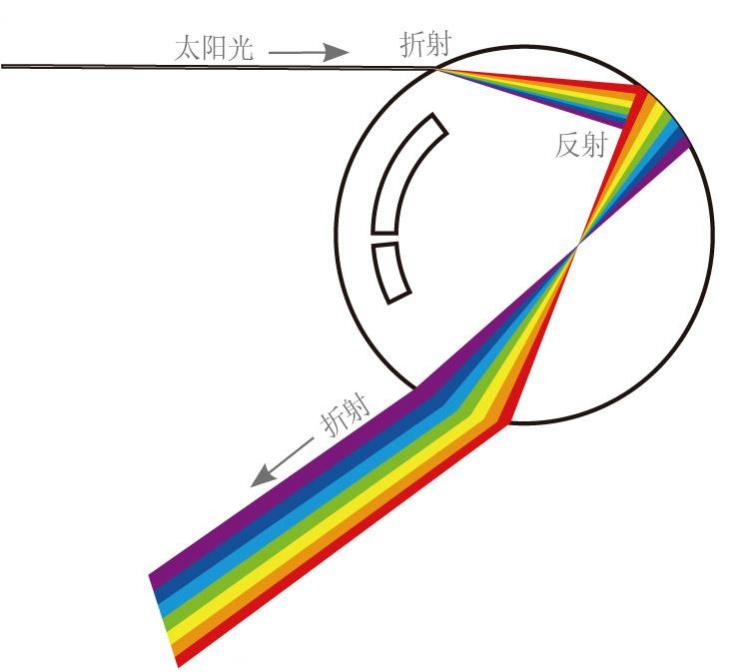
\includegraphics[width=0.7\textwidth]{c1_rainbow_02.jpg}
  \end{figure}
\end{frame}

\begin{frame}
  \frametitle{归纳法 | 解析彩虹}
  \begin{figure}
    \centering
    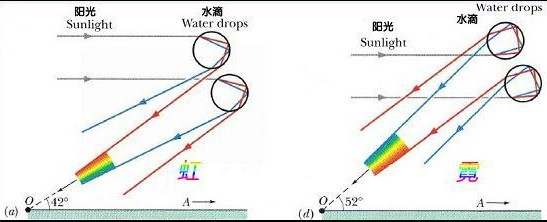
\includegraphics[width=\textwidth]{c1_rainbow_03.jpg}
  \end{figure}
\end{frame}

\begin{frame}
  \frametitle{归纳法 | 解析彩虹}
  \begin{block}{迪特里希的遗憾}
    \begin{itemize}
      \item 错误:彩虹上各种颜色产生取决于光线射入的深度和水的透明度
      \item 正确:不同颜色光的波长不同
      \item 番外:“破坏了彩虹的诗意”
    \end{itemize}
  \end{block}
\end{frame}

% 1-5,1604
\section{自由落体——头脑风暴}
\begin{frame}
  \frametitle{头脑风暴 | 自由落体}
  \begin{columns}
    \column{0.6\textwidth}
  \begin{block}{当时的科学}
    \begin{itemize}
      \item 亚里士多德的观点:做自由落体的物体的下落速度与质量成正比 
      \item 自然而然的推论:如果两块重量不等的石头自由坠落,较重的一块比较轻的一块落地更快
    \end{itemize}
  \end{block}
  \begin{block}{伽利略}
    \begin{itemize}
      \item 实验(?):比萨尔斜塔
      \item 思考:思维实验
    \end{itemize}
  \end{block}
    \column{0.4\textwidth}
    \begin{figure}
      \centering
      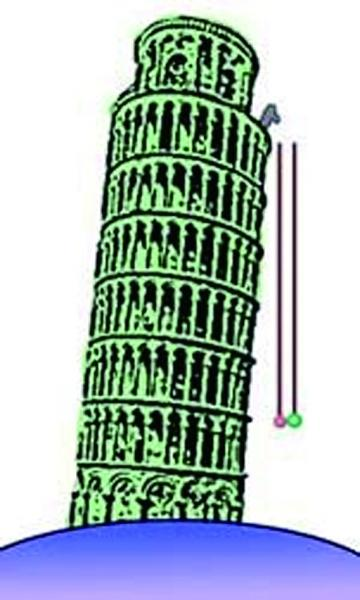
\includegraphics[width=0.9\textwidth]{c1_stone_01.jpg}
    \end{figure}
  \end{columns}
\end{frame}

\begin{frame}
  \frametitle{头脑风暴 | 自由落体}
  \begin{block}{伽利略的思维实验}
    \begin{itemize}
      \item 材料与方法:把较重的石头和较轻的石头绑在一起
      \pause
      \item 预期结果
        \begin{enumerate}
          \item 速度介于较快的速度和较慢的速度之间(两块石头互相掣肘)
          \item 速度比一块石头下落得快(两块石头绑在一起比一块石头重)
        \end{enumerate}
      \item 结论:亚里士多德的定律出现自相矛盾,不攻自破
      \item 推论:物体下落的速度与其重量无关(与空气阻力有关)
    \end{itemize}
  \end{block}
  \pause
  \begin{block}{\alert{归谬法}}
    \begin{itemize}
      \item 归谬法是一种论证方式,首先假设某命题成立,然后推理出矛盾、不符已知事实或荒谬难以接受的结果,从而下结论说某命题不成立。
      \item 反证法(又称背理法)是一种论证方式,它首先假设某命题不成立(即在原命题的条件下,结论不成立),然后推理出明显矛盾的结果,从而下结论说原假设不成立,原命题得证。
    \end{itemize}
  \end{block}
\end{frame}

% 1-232,1971
\begin{frame}
  \frametitle{头脑风暴 | 自由落体}
  \begin{block}{月球上的实验}
    \begin{itemize}
      \item 1971年,戴维\textbullet 斯科特
      \item 在没有空气的月球大气中,他同时放下一片羽毛和一把重量为羽毛的40倍的锤子,二者同时降落在月球表面
    \end{itemize}
  \end{block}
\end{frame}

% 1-25,1845
\section{多普勒效应——以音代光}
\begin{frame}
  \frametitle{以音代光 | 多普勒效应}
  \begin{block}{多普勒效应——光}
    \begin{itemize}
      \item 已知:光像波一样传播,彩色的出现是由于光波传播速度不同——紫光最快,红光最慢。
      \item 理论:(此前从未有人注意到)光源和观察者的活动也会发生作用
      \item 计算:达到每秒33英里(191,190 km/h)时才能用肉眼观察到这一效应
      \item 实验:无法在实验室里证明多普勒效应……
    \end{itemize}
  \end{block}
\end{frame}

\begin{frame}
  \frametitle{以音代光 | 多普勒效应}
    \begin{figure}
      \centering
      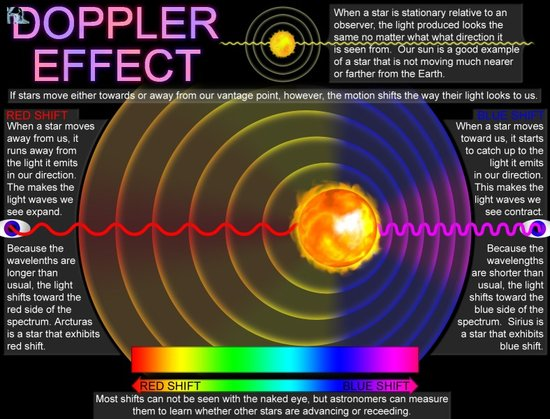
\includegraphics[width=0.8\textwidth]{c1_doppler_01.jpg}
    \end{figure}
\end{frame}

\begin{frame}
  \frametitle{以音代光 | 多普勒效应}
  \begin{block}{替代实验}
    \begin{itemize}
      \item 基础:声音也以波的形式向外传播,只是速度比光慢很多
      \item 推测:对光线所做的假想用于声音应该“完全地、严格地”符合
      \item 计算:把“7”音听成高半度的“1”音,需要声源以70 km/h的速度接近观察者
      \item 实验:自从蒸汽机车发明以来,70 km/h就在人们可以达到的范围之内
    \end{itemize}
    \vspace{-1.5em}
    \begin{figure}
      \centering
      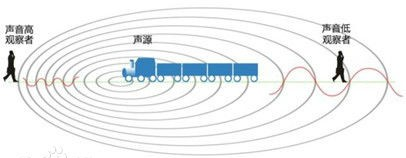
\includegraphics[width=0.8\textwidth]{c1_doppler_02.jpg}
    \end{figure}
  \end{block}
\end{frame}

\begin{frame}
  \frametitle{以音代光 | 多普勒效应}
  \begin{block}{铁道上的号手}
    \begin{itemize}
      \item 1845年,克里斯托弗\textbullet 拜斯\textbullet 巴洛特
      \item 材料一:机车的汽笛
        \begin{itemize}
          \item 优点:汽笛声音响亮,相距很远也能听见
          \item 缺点:预实验发现汽笛的声调很不纯正,乐师很难准确判定它的高低
        \end{itemize}
      \item 材料二:号手吹奏“5”音
      \item 设想非常简单:一位号手与两名协助者共同随车厢前进,其余号手分成3组等在轨道旁,每组间隔400米 
        \begin{itemize}
          \item 火车前行途中,车厢上的号手按实验要求吹奏“5”音,站在铁轨旁的乐手们各自记录音调的不同
          \item 火车回退时角色倒置:轨道边的号手吹奏,车厢上的乐师记录
        \end{itemize}
      \item 执行起来困难重重
        \begin{itemize}
          \item 火车越快,噪音越大,号声越不清楚;火车很慢,音调差别非常细微,难以辨别
          \item 速度确定在18-72 km/h,但司机无法保证匀速行驶
          \item 计划精准,但乐手们做不到在完全相符的时间内吹响小号
        \end{itemize}
    \end{itemize}
  \end{block}
\end{frame}

\begin{frame}
  \frametitle{以音代光 | 多普勒效应}
  \begin{block}{多普勒效应——声音}
    救护车靠近时,喇叭的音调变高,远离时就会变低。
  \end{block}
  \pause
  \begin{block}{多普勒效应的应用}
    \begin{itemize}
      \item 巴洛特的预见:唯一的可能就是“没准儿以后会造出更好的乐器来”
      \item 实际应用:飞机导航系统,宇宙大爆炸理论,雷达陷阱,天文、化学、医药等领域
    \end{itemize}
  \end{block}
\end{frame}

% 2-235,1994
\section{运动定律——直觉与科学}
\begin{frame}
  \frametitle{直觉与科学 | 运动定律 | 小测验}
  \begin{figure}
    \centering
    
\includegraphics[width=0.6\textwidth]{c1_test_03.jpg}
  \end{figure}
\end{frame}

\begin{frame}
  \frametitle{直觉与科学 | 运动定律 | 小测验(1/2)}
  \begin{figure}
    \centering
    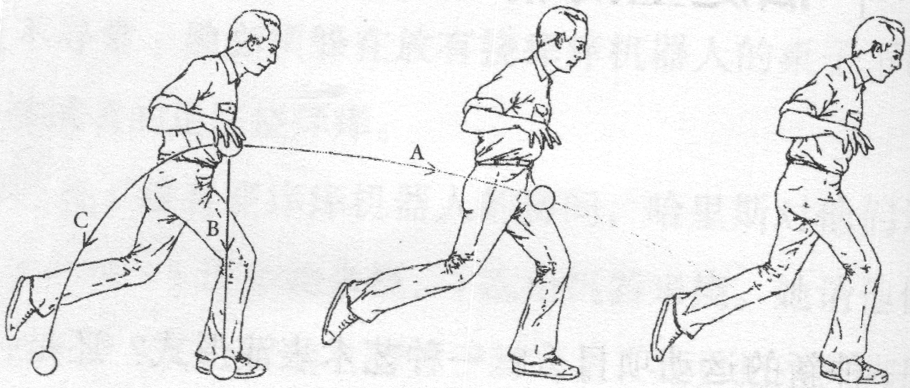
\includegraphics[width=0.9\textwidth]{c1_test_01.png}
  \end{figure}
\end{frame}

\begin{frame}
  \frametitle{直觉与科学 | 运动定律 | 小测验(2/2)}
  \begin{figure}
    \centering
    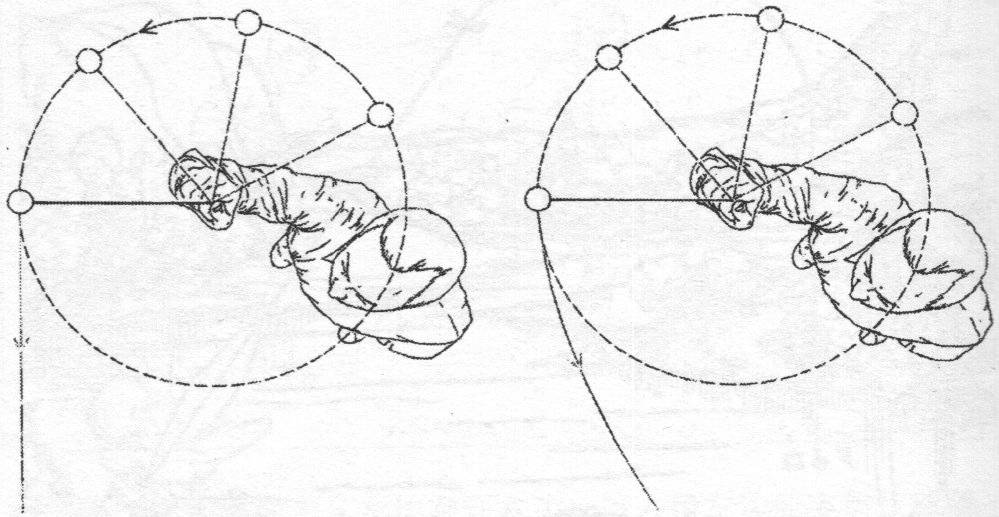
\includegraphics[width=0.9\textwidth]{c1_test_02.png}
  \end{figure}
\end{frame}

\begin{frame}
  \frametitle{直觉与科学 | 运动定律}
  \begin{block}{科学问题}
    具备不同物理学知识水平的人都是如何理解运动的。
  \end{block}
  \pause
  \begin{block}{冲力说}
    每个运动都必须由力来维持。冲力是球体中包含的力,维持球体的运动,只是与此同时,它会缓慢耗尽。一个物体停下来,是因为它内在的运动能量用尽了。
  \end{block}
  \pause
  \begin{block}{牛顿运动定律}
    \begin{itemize}
      \item 如果一个人在行进中让一个球落下,那么该球会沿着一条与人前进方向一致的曲线朝着地面运动。
      \item 如果没有力的作用,物体总是沿着直线运动的。
    \end{itemize}
  \end{block}
  \pause
  \begin{block}{教育学家}
    只有事先消除已有的错误想法,新知识才能得到有效的传授。
  \end{block}
\end{frame}

% 2-47,1911
\section{咖啡因——科学典范}
\begin{frame}
  \frametitle{科学典范 | 咖啡因}
  \begin{block}{可口可乐案件}
    \begin{itemize}
      \item 起因:美利坚合众国指控40大桶及20小桶可口可乐案(可口可乐中的咖啡因成分有毒且使人上瘾?)
      \pause
      \item 1911年,哈里\textbullet 霍林沃斯,5周时间,大规模实验
        \begin{itemize}
          \item 16名年龄在19-39岁的被试者
          \item 反复测试注意力、检验感知力、考问并评定判断力
          \item 做心算题、说出颜色名称、找出反义词
          \item “咖啡因组”(含有咖啡因的胶囊),“安慰剂对照组”(含有乳糖的胶囊)
          \item 从64000次测量中提取出一个清晰的供述,展示各种图形、表格
          \item 咖啡因:一种温和的兴奋剂(大量服用可能会影响睡眠)
        \end{itemize}
    \end{itemize}
  \end{block}
\end{frame}

\begin{frame}
  \frametitle{科学典范 | 咖啡因}
  \begin{block}{后续影响}
    \begin{itemize}
      \item 案件:没能对诉讼结果产生任何影响
      \item 霍林沃斯在极为有限的时间内进行了极为合理的科学实验,迄今为止,它仍被视为周密而可靠的典范。
      \item (妻子)莉塔\textbullet 霍林沃斯成功运用可口可乐实验的方法,令人信服地证明了——月经周期并不会影响女性的智力。(博士论文——《功能性的周期:通过实验研究女性在月经期间的智力及运动能力》)
    \end{itemize}
  \end{block}
\end{frame}

\section{史海撷华——真正的疯狂}
% 1-9,1758
\begin{frame}
  \frametitle{真正的疯狂 | 电}
  \begin{block}{哲学家的短袜}
    \begin{itemize}
      \item 1758年,罗伯特\textbullet 西默(“赤脚哲学家”),《哲学学报》
      \item 对“脱袜子噼噼啪啪响“这一现象以一种哲学的方式进行观察
      \pause
      \item 实验观察绝对充分
        \begin{itemize}
          \item 研究材料的普遍性——袜子
          \item 实验进行的极端简易性——穿上和脱掉袜子
        \end{itemize}
      \item 实验相当细致
        \begin{itemize}
          \item 曾3次在皇家协会的集会上讲解实验
          \item 报告细节丰富,长达30页,包括由此引起的启迪与思索
        \end{itemize}
      \item 结果与改进
        \begin{itemize}
          \item 测试棉袜、毛袜和丝袜后发现毛袜和丝袜最适宜做实验
          \item 毛袜穿在丝袜外面还是相反无关紧要
          \item 只用白色和黑丝的丝袜(反应最强烈)
          \item 把长袜套在手上(清洁,袜子可以用得更久)
        \end{itemize}
    \end{itemize}
  \end{block}
\end{frame}

% 1-11,1772
\begin{frame}
  \frametitle{真正的疯狂 | 电流}
  \begin{block}{电流下的宦官}
    \begin{itemize}
      \item 现象:用莱顿瓶给一列人通电,一些表演中电的影响在链条中部消失了
      \pause
      \item 猜想:断点处的年轻人“不具备男性特征所要求的一切”
      \item 实验:西戈\textbullet 德拉丰,国王的3个阉人乐师
      \item 结果:国王的宦官们并没有干扰链条中的电流,相反,他们看上去对于电击的反应更加敏感
      \item 原因:人们所站的地面的导电性
    \end{itemize}
  \end{block}
\end{frame}

% 2-14,1752
\begin{frame}
  \frametitle{真正的疯狂 | “闪”念}
  \begin{block}{富兰克林的风筝}
    \begin{itemize}
      \item 1752年,本杰明\textbullet 富兰克林,在雷雨天放飞风筝
      \item 想证明“天上的电”和“地上的电”是同一回事
      \item “人类做过的最勇敢的一次实验”!?
    \end{itemize}
    \vspace{-1.5em}
    \begin{figure}
      \centering
      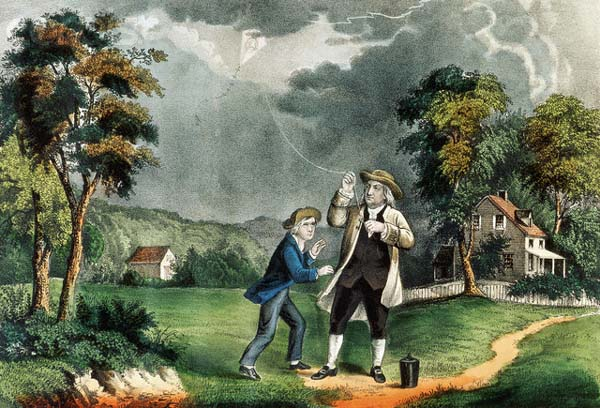
\includegraphics[width=0.7\textwidth]{c1_franklin_01.jpg}
    \end{figure}
  \end{block}
\end{frame}

% 2-39,1888
\begin{frame}
  \frametitle{真正的疯狂 | 电流之争}
  \begin{figure}
    \centering
    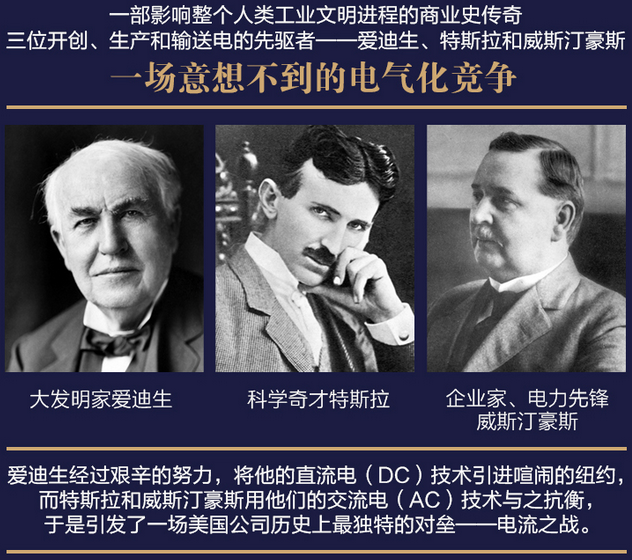
\includegraphics[width=0.75\textwidth]{c1_dc_ac_01.png}
  \end{figure}
\end{frame}

% 2-18,1758
\begin{frame}
  \frametitle{真正的疯狂 | 把油倒入水中}
  \begin{block}{航海——抑制波浪}
    \begin{itemize}
      \item 现象:用油来平息波浪
      \item 实验:富兰克林,阿沙尔,约翰\textbullet 希尔兹,海因里希\textbullet 徐讷福斯
    \end{itemize}
  \end{block}
  \pause
  \begin{block}{化学——单分子层}
    \begin{itemize}
      \item 现象:一滴油会“急速、剧烈地”在水面“扩散成很大一片”
      \item 应用:估算分子直径$\longrightarrow$ 解析甘油三油酸酯
    \end{itemize}
  \end{block}
  \pause
  \begin{block}{生物学——细胞膜}
    \begin{itemize}
      \item 现象:某些物质对细胞膜的穿透性与它们在橄榄油中的溶解性有着独特的关联
      \item 应用:找出了包裹细胞的薄膜的成分$\longrightarrow$血细胞的细胞膜一定有两个分子那么“厚”
    \end{itemize}
  \end{block}
\end{frame}

% 1-233,1971
\begin{frame}
  \frametitle{真正的疯狂 | 原子钟环球飞行}
  \begin{block}{狭义相对论}
    时间在不同的地方流逝的速度是不一样的,而是和物体运动的速度有关。运动快的物体,它的时间也就过得更慢。
  \end{block}
  \pause
  \begin{block}{广义相对论}
    时钟的快慢不仅与它的运动速度有关,也与重力有关。时钟在山顶上要比在山谷中走得快些。
  \end{block}
  \pause
  \begin{block}{原子钟环球飞行}
    \begin{itemize}
      \item 爱因斯坦的理论在日常生活中无法被证明:必须以接近光速的高速运动,或者使用足够精确的时钟
      \item 1971年,理查德\textbullet 基廷,约瑟夫\textbullet 海富勒,2只重60公斤的原子钟,波音747飞机
      \item “如果您想活得更久,您只需要向东飞。”(注:十亿分之一秒量级)——霍金
    \end{itemize}
  \end{block}
\end{frame}

% 1-261,1976
\begin{frame}
  \frametitle{真正的疯狂 | 火星生命}
  \begin{block}{生命——符合地球生命的构成原则}
    \begin{itemize}
      \item 生命是以碳元素为基础形成的。
      \item 地球生命的共同特征是新陈代谢,所有生命体都要从外界吸收养料并排除废物。
    \end{itemize}
  \end{block}
  \pause
  \begin{block}{火星生命?}
    \begin{itemize}
      \item 1976年,吉尔伯特\textbullet 莱温,“海盗1号”,火星土壤,喷洒含有放射性标记碳元素的营养剂
      \item 结果:逸出的气体带放射性
      \item 结论:土壤中的生命“吃掉”了营养剂并释放了废弃物?非生物的化学氧化反应?
    \end{itemize}
  \end{block}
\end{frame}

% 2-3,1654
\begin{frame}
  \frametitle{真正的疯狂 | 马德堡半球实验}
  \begin{block}{“真空”}
    \begin{itemize}
      \item “自然界厌恶真空”?
      \item “空气有重量”!
      \item 应用:吸管、吸尘器……
    \end{itemize}
  \begin{figure}
    \centering
    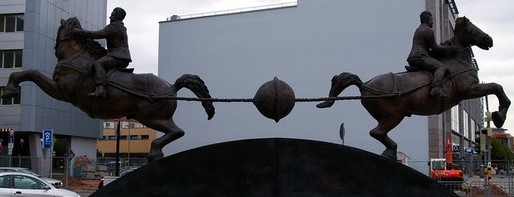
\includegraphics[width=0.9\textwidth]{c1_air_01.jpg}
  \end{figure}
  \end{block}
\end{frame}

% 2-29,1881
\begin{frame}
  \frametitle{真正的疯狂 | 最成功的失败实验}
  \begin{block}{以太}
    \begin{itemize}
      \item 每一种波都需要介质才能传播——声波需要空气,水波需要水,光波呢?(以太?)
      \item 1881年,阿尔伯特\textbullet 迈克尔逊(1907年,诺贝尔物理学奖),“干涉折光仪”;1887年,迈克尔逊、爱德华\textbullet 莫雷
      \item 目的:找到以太存在的证据
      \item 原理:“以太风”会影响光的传播(“顺风”,“逆风)——只需测出不同光线的速度差异,便可以证明以太的存在
      \item 策略:光速太快——通过某种方法直接算出两束光线的速度差异,无须确定各自光线的绝对速度
    \end{itemize}
  \end{block}
\end{frame}

\begin{frame}
  \frametitle{真正的疯狂 | 最成功的失败实验}
  \begin{block}{以太}
    \begin{itemize}
      \item 过程:两束光——一束光:“逆风”—“顺风”;另一束光:“侧风”—“侧风”
      \item 预期:第二束光永远是赢家(?)
      \item 结果:并未认出那一道光才是赢家,两束光总是同时回来
      \item 结论:唯一可能的解释——根本就没有以太
    \end{itemize}
  \end{block}
  \vspace{-0.5em}
  \begin{figure}
    \centering
    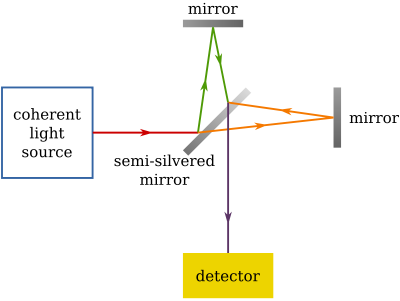
\includegraphics[width=0.45\textwidth]{c1_michelson_01.png}
  \end{figure}
\end{frame}

% 2-52,1927
\begin{frame}
  \frametitle{真正的疯狂 | 世上最无聊的实验}
  \begin{block}{沥青滴落实验}
    \begin{itemize}
      \item 1927年,托马斯\textbullet 帕奈尔,澳大利亚布里斯班市昆士兰大学
      \item 目的:测量极高黏度沥青在室温环境下的流动速度,演示沥青的某种已知特性,同时尝试发现沥青的新型特征
      \pause
      \item 1930(0)—1938.12(1)—1947.2(2)—1954.4(3)—1962.5(4)—1970.8(5)—1979.4(6)—1988.7(7)—2000.11.28(8)—2014.4.20(9)
      \item 结果:沥青的黏度大约是水的千亿倍
      \item 影响
        \begin{itemize}
          \item 2003年,“世界上持续时间最长的实验”——《吉尼斯世界纪录》
          \item 2005年,托马斯\textbullet 帕奈尔,约翰\textbullet 梅恩斯通,“搞笑诺贝尔奖”
          \item 2006年,网站——“网上最无聊的页面”
          \item “沥青滴落实验”乐团在聚友网发布三首单曲——《第一滴》、《第二滴》、《第三滴》
        \end{itemize}
    \end{itemize}
  \end{block}
\end{frame}

\begin{frame}
  \frametitle{真正的疯狂 | 世上最无聊的实验}
  \begin{block}{沥青滴落实验}
    \begin{figure}
      \centering
      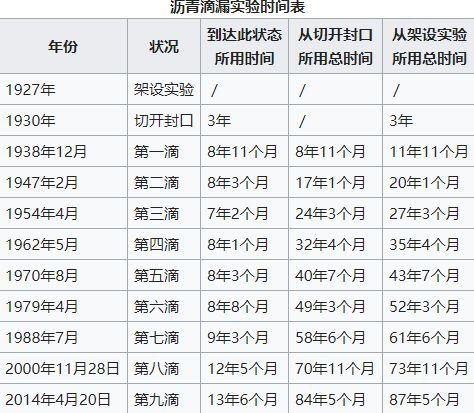
\includegraphics[width=0.65\textwidth]{c1_liqing.jpg}
    \end{figure}
  \end{block}
\end{frame}

% 2-117,1960
% 1-135,1951
\begin{frame}
  \frametitle{真正的疯狂 | 浴缸宇航员}
  \begin{block}{浴缸宇航员}
    \begin{itemize}
      \item 目的:研究失重状态对人体的影响(生理机能、饮食、睡眠……)
    \pause
      \item 卧床研究——10名男子躺着度过2个星期,不理想
      \item 解决方案——水,在地球上水能够最好地模拟无重力状态
      \item 1960.1.27—2.3,杜安\textbullet 格拉韦林(“浴缸里的上尉”),长2米、宽1米的水箱
      \item 结果:每一天格拉韦林都觉得爬出浴缸变得更加困难
      \item 实验完善——带上防水头盔,完全在水下度过数日
      \item 1986年,鲍里斯\textbullet 莫鲁科夫,持续时间最长(一年)的卧床研究
    \end{itemize}
  \end{block}
  \pause
  \begin{block}{眩晕轰炸机}
    \begin{itemize}
      \item 人在空气中以何种方式坠落,并不影响其失重状态。
      \item 时至今日,飞机的抛物线飞行是在地球重力场制造长达半分钟失重状态的唯一途径。
    \end{itemize}
  \end{block}
\end{frame}

% 2-175,1975
\begin{frame}
  \frametitle{真正的疯狂 | 刮擦黑板声}
  \begin{block}{刮擦黑板声的听觉效应}
    \begin{itemize}
      \item 1975年,大卫\textbullet 伊莱
      \item 现象:刮擦黑板声——难以忍受,耳朵疼痛,鸡皮疙瘩,冒冷汗……原因为何?
    \pause
      \item 猜想:不是噪音本身,而是对其产生过程的想象
      \item 实验:16位被试者(一部分知情,一部分不知情),刮擦黑板声(实验)和无害音组成的音列(对照),记录皮肤电阻(人体兴奋程度的度量指标)
      \item 结果:有时知情组被试者的皮肤电阻更高,有时却是不知情组的数值更高
    \end{itemize}
  \end{block}
\end{frame}

% 2-192,1986
\begin{frame}
  \frametitle{真正的疯狂 | 刮擦黑板声——续}
  \begin{block}{一把园艺镰刀在石板上的缓慢刮擦}
    \begin{itemize}
      \item 实验1:24名被试者,16种声音,记录被试者的评价,筛选出得分最差的声音
      \item 实验2:合成“人造数字版本”的镰刀刮擦声,同样令人难以忍受
      \item 假设:过高的频率
      \item 实验3:降低高频——结果依旧(意外发现:低频部分缺失时,声音变得可以忍受了)
      \item 猜想
        \begin{itemize}
          \item 这种声音与猕猴发出的示警叫声相似
          \item 条件反射(人们想象着手指甲刮过黑板时令人不适的触感,才会产生这种强烈的反应)
        \end{itemize}
      \item 获奖:2006年,搞笑诺贝尔奖,哈尔彭、布雷克、希伦布兰德
    \end{itemize}
  \end{block}
\end{frame}

% 1-252,1975
\begin{frame}
  \frametitle{真正的疯狂 | 汗液提取物}
  \begin{block}{候诊室里的汗液提取物}
    \begin{itemize}
      \item 生物学家:许多动物之间通过易于扩散的性吸引物质配对
      \item 心理学家:人类已经进化得太高等,这种低级的影响没有作用
    \pause
      \item 实验
        \begin{itemize}
          \item 雄烯二酮(男子腋下汗液的一种提取物)
          \item 迈克尔\textbullet 柯克—史密斯(实验设计),不知道实验目的的助手(负责记录)
          \item 开始4天仅观察,接下来的5周,喷洒雄烯二酮
        \end{itemize}
      \item 结果结论
        \begin{itemize}
          \item 在人类选择配偶的过程中,荷尔蒙也是起很大作用的。
          \item 雄烯二酮的作用是很微弱的,而且很可能被许多其他因素掩盖效果
        \end{itemize}
      \item 后续影响
        \begin{itemize}
          \item 把雄烯二酮兑到神秘香水里
          \item BBC在隐秘摄像机的拍摄下重做实验
        \end{itemize}
    \end{itemize}
  \end{block}
\end{frame}

% 1-46,1899
\begin{frame}
  \frametitle{真正的疯狂 | 尸体腐败}
  \begin{block}{菜园里的尸体}
    \begin{itemize}
      \item 课题:“尸体动物群”学说
      \item 材料:死婴,牛、猫、狐狸、老鼠、鼹鼠的腐尸
      \item 问题
        \begin{itemize}
          \item 尸体昆虫是以什么样的顺序在一具死尸上进行繁殖的?
          \item 人类尸体上的昆虫与动物尸体上的昆虫有无不同?
          \item 季节对尸体动物群有何影响?
          \item 一具尸体从被腐蚀到只剩下骨头需要多长时间?
        \end{itemize}
      \item 应用
        \begin{itemize}
          \item 对于尸体上昆虫繁殖顺序的了解关系到死亡时间的确定
          \item 法庭昆虫学已经成为犯罪侦查学的一个分支
        \end{itemize}
    \end{itemize}
  \end{block}
\end{frame}

% 2-214,1992
\begin{frame}
  \frametitle{真正的疯狂 | 尸体腐败}
  \begin{block}{死鲸沉没}
    \begin{itemize}
      \item 1992年,克雷格\textbullet 史密斯
      \item 课题:当大块有机材料沉没时,深海里到底会发生什么
      \item 材料:死鲸
      \item 实验:寻找鲸尸体,让死鲸沉没,申请资金,潜艇下潜观察,鲨鱼威胁,……
      \item 推测:某种物种完全只以鲸尸体为食(80年,16千米)
    \end{itemize}
  \end{block}
\end{frame}

% 2-227,1993
\begin{frame}
  \frametitle{真正的疯狂 | 尸体腐败}
  \begin{block}{尸体农场}
    \begin{itemize}
      \item 问题
        \begin{itemize}
          \item 胳膊经过多久才会掉下来?
          \item 牙齿什么时候从头骨上脱落?
          \item 昆虫以何种顺序在尸体上繁殖?
          \item 从一具躯体变为只剩骨架需要多长时间?
        \end{itemize}
      \item 1981年,比尔\textbullet 巴斯,人类学研究机构(“尸体农场”)
      \item 1993年,帕特丽夏\textbullet 康韦尔,惊悚罪案小说《尸体农场》
    \end{itemize}
  \end{block}
\end{frame}

% 2-218,1992
\begin{frame}
  \frametitle{真正的疯狂 | 水面飞驰}
  \begin{block}{耶稣蜥蜴如何在水面飞驰}
    \pause
    \begin{itemize}
      \item 1992年,詹姆斯\textbullet 格拉希恩
      \item 材料:耶稣蜥蜴——亲自到原始森林去寻找
      \item 其他:饲养蜥蜴,架设大水盆,高速摄像机,流体力学理论,……
      \item 原理:拍打水面——表面张力的反作用力——压出气囊
      \item 人:80 kg,110 km/h
    \end{itemize}
  \end{block}
\end{frame}

% 2-275,2003
\begin{frame}
  \frametitle{真正的疯狂 | 在糖浆里游泳}
  \begin{block}{黏滞度对游泳的影响}
    \begin{itemize}
      \item 问题:在糖浆里游泳比在水里更快、更慢还是速度相当?
    \pause
      \item 历史悠久:自17世纪以来400年
        \begin{itemize}
          \item 牛顿:速度更慢
          \item 惠更斯:液体的黏滞度不会带来任何影响
        \end{itemize}
      \item 2003年,艾德\textbullet 喀斯勒、布莱恩盖\textbullet 特芬格
      \item 准备:22份批准书,材料(凝结剂),搅拌均匀
      \item 实验:9位竞技游泳选手,6位业余游泳选手,25米水—50米糖浆—25米水
      \item 结果:游泳者在水和糖浆里的速度基本一样
      \item 解释:阻力更大、推力也更大,两个力增加的强度相等,因此相互抵消
      \item 获奖:2005年,搞笑诺贝尔化学奖
    \end{itemize}
  \end{block}
\end{frame}

\begin{frame}
  \frametitle{疯狂的实验 | 总结}
  \begin{block}{科学的方法}
    \begin{itemize}
      \item 方法:归纳法、归谬法、替代法、逆向思维
      \item 实验:对照实验、双盲实验
    \end{itemize}
  \end{block}
  \pause
  \begin{block}{科学的真相}
    \begin{itemize}
      \item 空想容易实干难
      \item 结果有趣过程枯燥
      \item “智慧简单又不简单”
      \item 大胆、细心、严谨、耐心
      \item 科学没有贵贱之分,但科学家有善恶之别
    \end{itemize}
  \end{block}
\end{frame}



\section*{Acknowledgements}
\begin{frame}
  \frametitle{Powered by}
  \begin{center}
    
\includegraphics[width=9cm]{power.png}
  \end{center}
\end{frame}

\end{document}

